\chapter{Project Work}\label{final}

\section{\ Data Description}
  \par In our project, we have used two datasets. One being the details of customers of a bank in Taiwan which has 24 attributes like the amount of given credit, gender of the person, education, marital status, age and history of past payments. The dataset has 30000 instances and was collected in 2005.~\cite{yeh2009comparisons}\par
  The second dataset consists of transactions made by credit cards in September 2013 by European credit card holders. There are over 284 thousand instances out of which 492 were frauds. The dataset consists of only numerical input variables which is a result of Principal Component Analysis and only two attributes could not be changed which are time and amount. ~\cite{dal2015calibrating}
\section{ Data Analysis}
	\par The first dataset on analysis showed that approximately 70 \% data corresponds to non default transactions and 30\% corresponded to defaulted transactions (shown in Fig 1). This is a bit skewed data but it can be neglected and our algorithms can be applied.\\
\begin{figure}
  \centering
  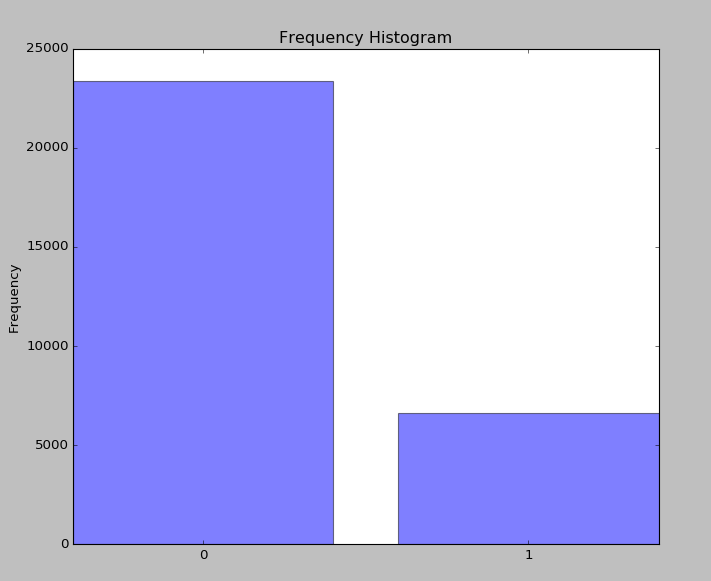
\includegraphics[scale=.4]{data1freq.png}
  \caption{Frequency Historgram of first dataset}
  
\end{figure}
\begin{figure}
  \centering
  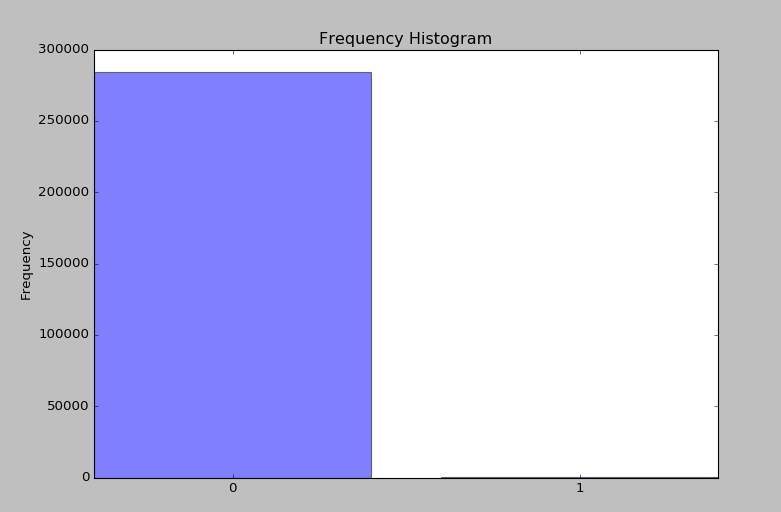
\includegraphics[scale=.4]{freq2init.png}
  \caption{Frequency Historgram of Second dataset before resampling}
  
\end{figure}
	The second dataset on the other hand was highly skewed with only 492 out of 2,84,000 being defaulted transactions. That amounts to .2\% of data being "1" and others being "0"(shown in Fig 2). This much skewedness had to be handled as just predicting "0" gives us an accuracy of 99.8\% but we have predicted all defaulted transations wrong which is a very big problem. To address this skewedness, we need to come up with few techniques. The techniques which we can use to resample are
\begin{enumerate}
	\item Collecting more data (which is not possible now)
	\item Over-Sampling, which is adding copies of underrepresented class
	\item Under-Sampling, which is removing copies of overrepresented class
	\item SMOTE- Synthetic Minority Over-Sampling Technique which is a mixture of both Under and Over Sampling.
\end{enumerate}
	\par We tried Under-Sampling wherein we randomly removed the "0"s and reduced the total instances to around 1350. Now the "1"s represented approximately 35\% of dataset [Refer Fig 3 for clearer analysis].
\begin{figure}
  \centering
  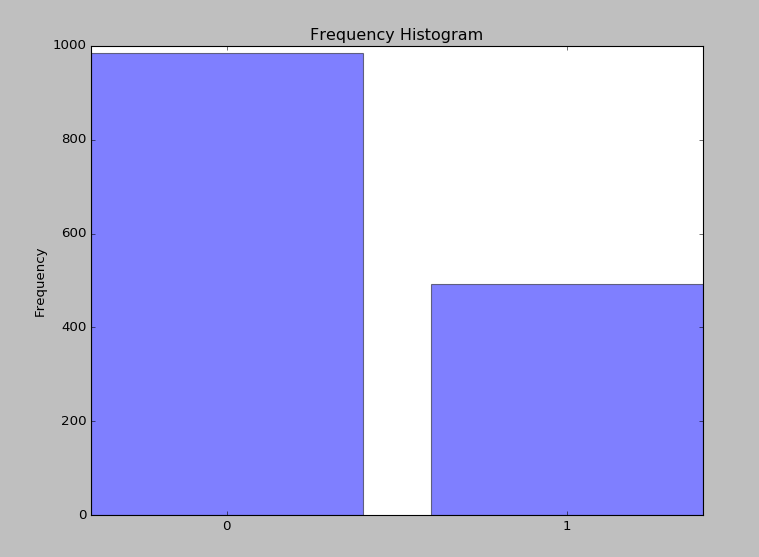
\includegraphics[scale=.4]{freq2fin.png}
  \caption{Frequency Histogram of Second dataset after resampling}
  
\end{figure}

   Thus after resampling, we can apply our machine learning algorithms for the second dataset and find our results. To analyse further, we decided to apply our machine learning algorithms on the dataset before Under-Sampling so that we check our efficiency in predicting the "1"s. Now we'll discuss the algorithms and techniques we applied and compare them for both datasets.For every algorithm, we have used 70\% of training data for training and rest 30\% for the testing of our model.

\section{ Logistic Regression } 
\par In Machine Learning, logistic regression is a statistical method wherein we try to approximate the hypothesis by minimising the cost associated with the hypothesis.In this form of regressive analysis, we approximate the hypothesis to be a linear model of the features (independent variables). Logistic Regression is used for predicting binary dependent variables rather than a continuous outcome. Here in our project the binary dependent variable is that the credit has been defaulted or not. If not defaulted the binary variable is '0' else the binary variable is '1'. ~\cite{al2002using}

In this algorithm, here $x_{ij}$ are the features and $y_{i}$  is the result for the corresponding training data ($i$ ranges from $[1,\text{Number of instances}]$ and $j$ ranges from $[1,\text{Number of attributes}]$ ). Now we assume \begin{center} 
 $p_{\theta}(x) = \Sigma \theta_{i}x_{i}$ ~\cite{Stanford} \\ $p_{\theta}(x) = \theta^{T}x $ ~\cite{Stanford}\end{center} (ie) linear function of $x_{i}$ where  $p_{\theta}(x)$ is the prediction . Now in our classification problem $y$ can only be 1 or 0. So to correct the $y$, we introduce a Sigmoid function \begin{center}$q(x) = \frac{1}{1+e^{-x}}$ ~\cite{Stanford}\end{center}. The speciality of the function is it's range is $[0,1]$ and with the value of 0.5 at $x=0$.
 Now is we replace  $p_{\theta}(x)$  as \begin{center}
 $p_{\theta}(x) = q(\theta^{T}x)$~\cite{Stanford}
 \end{center}
 We initialise all $\theta_{i}$ to $0$ initially. Now let the cost function \begin{center}
 $W(y |x;\theta ) = (p_{\theta}(x))^{y}(1-p_{\theta}(x))^{1-y} $ ~\cite{Stanford}
 \end{center}.
	This function $W(y)$ tries to convey the difference between our prediction for the training data and the actual value. Now to fit the $\theta$ , we will maximise the likelihood \begin{center}
	$J(\theta)= \Pi_{i=1}^{m}  W(y |x;\theta) $ ~\cite{Stanford}
	\end{center}
  	We know it is better to maximise the log likelihood. Thus taking log \begin{center}
  	$log(B(\theta)) = \Sigma_{i=1}^{m} y^{(i)}log(p(x^{(i)})) + (1-y^{(i)})log(1-p(x^{(i)}))$
  	\end{center}
   To maximise the log likelihood, we use the \textbf{Gradient Descent} algorithm which is \\
   Repeat until convergence \{  \begin{center}
   $\theta_{j} := \theta_{j} + \alpha \frac{\partial log(B(\theta))}{\partial \theta_{j}}$ (for every $j$) \end{center}
   \} \\
   Here $\alpha$ is called learning rate and by differentiating we get,
   \begin{center}
   $\theta_{j} := \theta_{j} + \alpha ( y-p_{\theta}(x))x$  (for
   every $j$) ~\cite{Stanford}
   \end{center}
 Implementing this algorithm, we get results(classification report) as shown below for dataset 1
\begin{center}
\begin{tabular}{| c | c | c | c | c |}
\hline
    & Precision & Recall & f1-score \\
\hline
0 & 0.83 & 0.98 & 0.90 \\
\hline
1 & 0.72 & 0.21 & 0.33 \\
\hline
avg & 0.81 & 0.82 & 0.78 \\
\hline
\end{tabular}
\end{center} 
\begin{center}
The accuracy is 82.25%.
\end{center}
 The results for the dataset 2 before resampling
\begin{center}
\begin{tabular}{| c | c | c | c | c |}
\hline
    & Precision & Recall & f1-score\\
\hline
0 & 1.0 & 1.0 & 1.0 \\
\hline
1 & 0.75 & 0.56 & 0.65 \\
\hline
avg & 1.0 & 1.0 & 1.0 \\
\hline
\end{tabular}
\end{center}
\begin{center}
The accuracy is 92.92%.
\end{center} 
 This table has to be analysed carefully. It says that the f1-score is 1.0 but the main thing is the data set is highly skewed. Instead from this table,if we consider the the f1-score of predicting "1"s , it gives us an f1-score of 0.65 which seems to be a bit legitimate score and we can consider this to be our result.\par
 Next the results for the second dataset after Under-Sampling
 \begin{center}
\begin{tabular}{| c | c | c | c | c |}
\hline
    & Precision & Recall & f1-score \\
\hline
0 & 0.96 & 0.99 & 0.97 \\
\hline
1 & 0.97 & 0.92 & 0.94 \\
\hline
avg & 0.96 & 0.96 & 0.96 \\
\hline
\end{tabular}
\end{center} 
\begin{center}
The accuracy is 95.17%.
\end{center}
After application of Under-Sampling, the absolute values of f1-score has decreased(which had to happen) and we get a f1-score of .98 which is very good score for this problem.
\section{ Neural Networks}
\par Neural Networks is machine learning algorithm used for non-linear classification. Basically, if we want to take into consideration two degree terms(e.g. $X_{1}^{2},X_{1}X_{2},X_{1}X_{3},X_{2}^{2}$) as features, we will have to consider $n^{2}$ two degree terms. This will lead to tremendous increase in number of features and applying gradient descent algorithm to minimise cost function will be very costly(in terms of computations). In Neural Networks we consider hidden layers between input and output layer, for the each unit in the layer there is a mapping from each unit of previous layer having a particular weightage. ~\cite{maind2014research}
\par In this algorithm, we randomly initialise the mapping terms so called $\theta_{ij}^{l}$ terms ($l$ is the layer from which mapping is done, $i$ is the cell from which mapping is done and $j$ is the cell to which mapping is done in $(i+1)^{th}$ layer). Compute the terms in next layer and so on until the output layer. We calculate the cost function using the predicted output. The error in output helps in calculating errors from previous layer which further helps in calculating error from previous layers. These errors are used while calculating gradient of cost function with $\theta_{ij}^{l}$. Gradient Descent method is used to optimise cost function. In each such iteration of forward and backward propagation we improve the values of $\theta_{ij}^{l}$ and so the output. ~\cite{maind2014research}
\begin{figure}
  \centering
  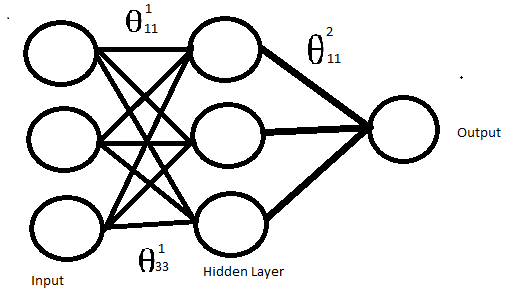
\includegraphics[scale=1]{Capture.png}
  \caption{Neural Networks}
\end{figure}
Implementing this algorithm, we get results(classification report) as shown below for dataset 1
\begin{center}
\begin{tabular}{| c | c | c | c | c |}
\hline
    & Precision & Recall & f1-score \\
\hline
0 & 0.82 & 0.98 & 0.90 \\
\hline
1 & 0.72 & 0.17 & 0.27 \\
\hline
avg & 0.80 & 0.82 & 0.77 \\
\hline
\end{tabular}
\end{center} 
\begin{center}
The accuracy is 81.66%.
\end{center}
The results for the dataset 2 before resampling
\begin{center}
\begin{tabular}{| c | c | c | c | c |}
\hline
    & Precision & Recall & f1-score \\
\hline
0 & 1.0 & 1.0 & 1.0\\
\hline
1 & 0.96 & 0.70 & 0.81\\
\hline
avg & 1.0 & 1.0 & 1.0 \\
\hline
\end{tabular}
\end{center}
\begin{center}
The accuracy is 99.95%.
\end{center} 
 This table has to be analysed carefully. It says that the f1-score is 1.0 but the main thing is the data set is highly skewed. Instead from this table,if we consider the the f1-score of predicting "1"s , it gives us an f1-score of 0.65 which seems to be a bit legitimate score and we can consider this to be our result.\par
 Next the results for the second dataset after Under-Sampling
 \begin{center}
\begin{tabular}{| c | c | c | c | c |}
\hline
    & Precision & Recall & f1-score \\
\hline
0 & 0.96 & 0.96 & 0.96 \\
\hline
1 & 0.93 & 0.93 & 0.93 \\
\hline
avg & 0.95 & 0.95 & 0.95\\
\hline 
\end{tabular}
\end{center}
\begin{center}
The accuracy is 95.21%.
\end{center} 
\section{ Naive Bayesian Algorithm}
  It is a Machine Learning technique based on Bayes theorem with an assumption of independence among predictors. Naive Bayesian technique assumes that all the features are independent of each other. Bayes theorem mathematically implies\begin{center}
  $P(A|B) = \frac{P(B|A) P(A)}{P(B)}$ ~\cite{rish2001empirical}
  \end{center}
  where \\
  $P(A|B)$ is the probability that event A occurs given event B\\
  $P(A)$ is the probability of occurence of event A\\
  $P(B)$ is the probability of occurence of event A\\
  $P(A|B)$ is the probability that event B occurs given event A\par
Now here $A$ will be the event that $y$ be "1" or "0". and $B$ be the events that each of the features have taken the value $x_{ij}$ (ie) for each instance in the test data, we will find the probability of it being 1 and the probability of it being 0 given all the $x_{ij}$ have occured. Then the assign $y=1$ if probability of "1" is larger ,else "0". The question now arises is how to calculate the probability?\par
  Now if the features take discrete values, we can then find the probability from the formula \begin{center}
  $P(A)= \frac{cnt(A)}{totalcnt}$
\end{center}
 But if the data is continuous instead of discrete, we apply some standard probability functions. Here we will use Gaussian(Normal) Probability distribution function for the prediction of probability.\begin{center}
	$P(x) = \frac{1}{\sqrt{2\sigma^{2}\pi}}e^{\frac{(x-\mu)^{2}}{\sqrt{2}\sigma}}$
\end{center}
Here \\$P(x)$ is the probability of $x$\\ $\mu$ is the Mean of the instances \\ $\sigma$ is the Standard Deviation of the instances. ~\cite{rish2001empirical}
\par Now we implement this algorithm for dataset 1 and find the following results.
\begin{center}
\begin{tabular}{| c | c | c | c | c |}
\hline
    & Precision & Recall & f1-score \\
\hline
0 & 0.79 & 0.98 & 0.90 \\
\hline
1 & 0.72 & 0.21 & 0.33 \\
\hline
avg & 0.81 & 0.82 & 0.78 \\
\hline
\end{tabular}
\end{center}
\begin{center}
The accuracy is 75.07%.
\end{center} 
Now when we implemented this algorithm for the algorithm for the second dataset before the application of Under-Sampling, we got the following results.

\begin{center}
\begin{tabular}{| c | c | c | c | c |}
\hline
    & Precision & Recall & f1-score\\
\hline
0 & 0.98 & 1.00 & 0.99 \\
\hline
1 & 0.80 & 0.04 & 0.08 \\
\hline
avg & 0.97 & 0.98 & 0.97 \\
\hline
\end{tabular}
\end{center}
\begin{center}
The accuracy is 97.77%.
\end{center}
\par What must be viewed here is that the data is skewed and our algorithm is working very poorly in predicting the default conditions.
\par Now after we apply Under-Sampling, we got the following results.

\begin{center}
\begin{tabular}{| c | c | c | c | c |}
\hline
    & Precision & Recall & f1-score \\
\hline
0 & 0.96 & 0.94 & 0.95 \\
\hline
1 & 0.88 & 0.93 & 0.90 \\
\hline
avg & 0.94 & 0.94 & 0.94 \\
\hline
\end{tabular}
\end{center}
\begin{center}
The accuracy is 94.05%.
\end{center}
Although the overall average has been decreased but we have succeeded in predicting fraud cases quite well and this model will be quite successful.
\section{ K-Nearest Neighbours}
\par $K$-nearest neighbours is machine learning algorithm widely used for classification problems. As the name suggests, to classify an test example, we compute it's distance from all the training examples. And divide the distances into different sets corresponding to the set which training sample belongs. The set which has least sum of $k$ smallest distances will be the required classification for the sample.
Here
\begin{center}
	$distance_{j}^{2} = \Sigma_{i=1}^{m}( Train_{ij} - Test_{i} )^{2} $\\	
\end{center}
where $distance_{j}$ represents distance of test example with the $j^{th}$ training example.\\
$m$ represents the number of features in the dataset\\
$Train_{ij}$ represents $i^{th}$ feature of the $j^{th}$ training example\\
$Test_{i}$ represents $i^{th}$ feature of test example.


\par How we choose value $k$?
Initially, error starts decreasing by increasing value of k until a value comes which has the least error and then again error starts increasing with increasing value of k. If we test on training sample itself error will increase on increasing value of k from beginning itself. ~\cite{guo2003knn}
 \par Results for Dataset 1.
\begin{center}
\begin{tabular}{| c | c | c | c | c |}
\hline
    & Precision & Recall & f1-score \\
\hline
0 & 0.84 & 0.97 & 0.90 \\
\hline
1 & 0.68 & 0.29 & 0.40 \\
\hline
avg & 0.81 & 0.83 & 0.80 \\
\hline
\end{tabular}
\end{center}
\begin{center}
The accuracy is 82.76%.
\end{center}
Now when we implemented this algorithm for the algorithm for the second dataset before the application of Under-Sampling, we got the following results.

\begin{center}
\begin{tabular}{| c | c | c | c | c |}
\hline
    & Precision & Recall & f1-score \\
\hline
0 & 1.00 & 1.00 & 1.00 \\
\hline
1 & 0.96 & 0.73 & 0.83 \\
\hline
avg & 1.00 & 1.00 & 1.00 \\
\hline
\end{tabular}
\end{center}
\begin{center}
The accuracy is 99.96%.
\end{center}
\par What must be viewed here is that the data is skewed and our algorithm is working very poorly in predicting the default conditions.
\par Now after we apply Under-Sampling, we got the following results.

\begin{center}
\begin{tabular}{| c | c | c | c | c |}
\hline
    & Precision & Recall & f1-score \\
\hline
0 & 0.92 & 0.99 & 0.96 \\
\hline
1 & 0.98 & 0.84 & 0.90 \\
\hline
avg & 0.94 & 0.94 & 0.94 \\
\hline
\end{tabular}
\end{center}
\begin{center}
The accuracy is 94.01%.
\end{center}
Although the overall average has been decreased but we have succeeded in predicting fraud cases quite well and this model will be quite successful.

\section{ Decision Trees}
\par Decision trees build regression models based on a structure of the tree. In Machine Learning, the decision is about a single predictor (attributes). In this algorithm, the main concept is to choose an attribute and make decisions on that and distribute the dataset according to the decision. Then recursively on the distributed datasets apply decisions on the other attributes and finally we reach a point that the dataset becomes completely homogeneous in one category.
\par The task is tough because we don't know upon which attribute the first decision has to be taken. Thus we solve this greedily. Our final destination is smaller and more homogeneous datasets. Thus at every step, we will try to maximise the homogeneity of the resulting datasets. Here the measure of homogeneity mathematically is the entropy of the dataset. In order to increase the homogeneity, we need to reduce to entropy of the datasets. Thus we have entropy of a random variable $X$ ~\cite{decisiontree}
\begin{center}
    $Entropy(X) = -\sum  P(x_{k})\log_2 P(x_{k}) $  ~\cite{decisiontree}
\end{center}
where $x_k$ are the values of the random variable $X$.\\
$P(x_k)$ is the probability of the occurence of $x_{k}$ for the variable $X$.
\par Thus we take the initial dataset, find it's entropy. Divide the dataset according to every attribute available and then find the resulting entropy. The attribute which results with the least entropy is then chosen and the dataset is divided accordingly.Then the datasets which are formed from the above said action are solved recursively.

Now for the results of this technique.

\begin{center}
\begin{tabular}{| c | c | c | c | c |}
\hline
    & Precision & Recall & f1-score \\
\hline
0 & 0.96 & 0.85 & 0.90 \\
\hline
1 & 0.34 & 0.67 & 0.45 \\
\hline
avg & 0.89 & 0.83 & 0.85 \\
\hline
\end{tabular}
\end{center}
\begin{center}
The accuracy is 82.25%.
\end{center}
Now when we implemented this algorithm for the algorithm for the second dataset before the application of Under-Sampling, we got the following results.

\begin{center}
\begin{tabular}{| c | c | c | c | c |}
\hline
    & Precision & Recall & f1-score \\
\hline
0 & 1.00 & 1.00 & 1.00 \\
\hline
1 & 0.64 & 0.67 & 0.65 \\
\hline
avg & 1.00 & 1.00 & 1.00 \\
\hline
\end{tabular}
\end{center} 
\par What must be viewed here is that the data is skewed and our algorithm is working very poorly in predicting the default conditions.
\par Now after we apply Under-Sampling, we got the following results.

\begin{center}
\begin{tabular}{| c | c | c | c | c |}
\hline
    & Precision & Recall & f1-score \\
\hline
0 & 0.95 & 0.93 & 0.94 \\
\hline
1 & 0.88 & 0.91 & 0.89 \\
\hline
avg & 0.93 & 0.93 & 0.93 \\
\hline
\end{tabular}
\end{center}
Although the overall average has been decreased but we have succeeded in predicting fraud cases quite well and this model will be quite successful.
\section{ Support Vector Machines}
SVM is a supervised learning algorithm. It is used to classify our data in positive and negative sets.
Given a set of data, we need a separating plane that divides the data in two sets, specifically our classes.(Refer Fig 5)
\begin{figure}
  \centering
  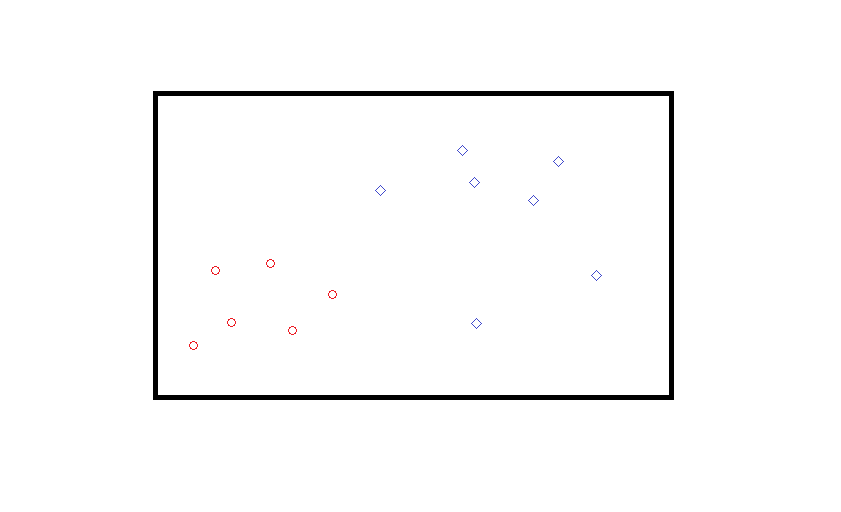
\includegraphics[scale=0.6]{kachra.png}
  \caption{Positive and Negative data sets}
  
\end{figure}

A hyperplane divides the given data into two classes. It can be a point, line, plane or hyperplane, depending upon whether the data is in one dimension, two dimension, three or more.(Refer Fig 6)
It seems very clear that there may be many such hyperplanes separating our data. So our task lies down at choosing one such hyperplane which gives best results.~\cite{svm}

\begin{figure}
  \centering
  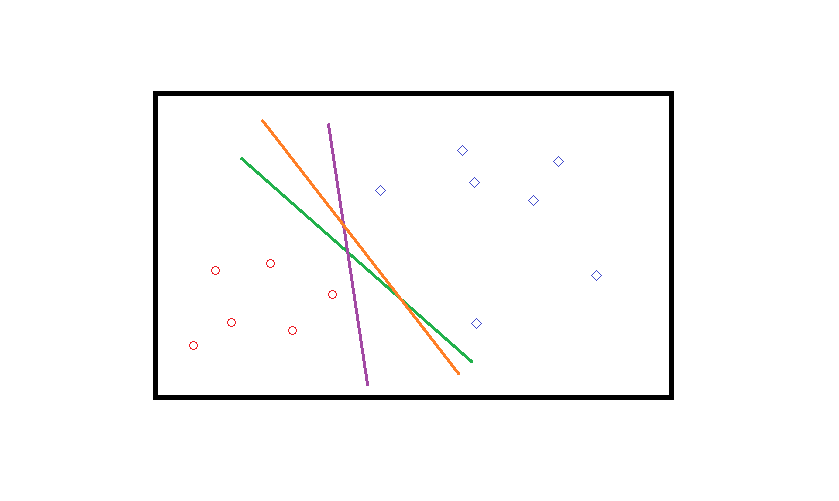
\includegraphics[scale=.6]{kachra1.png}
  \caption{Separating Hyperplanes ~\cite{svm}}
  
\end{figure}

The distance between the hyperplane and the closest point to the hyperplane is defined as the Margin. Clearly, no point lies inside the margin.(refer Fig 7)

\begin{figure}
  \centering
  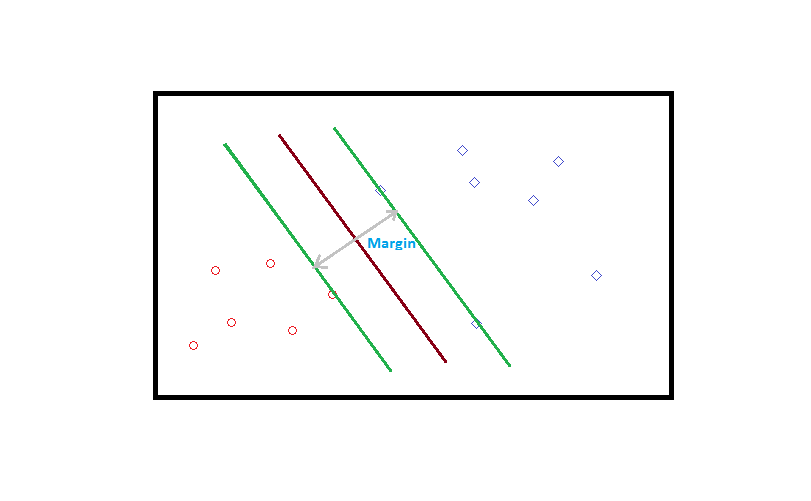
\includegraphics[scale=.6]{kachra2.png}
  \caption{Margin ~\cite{svm}}
  
\end{figure}

The hyperplane which has the largest margin is chosen and it eventually gives the best result.

As we saw in logistic regression, we chose a decision boundary by our constraint $$\displaystyle \min_\theta  \sum (y_i\log (h_\theta (i))+(1-y_i)\log(1-h_\theta (i))) $$.

If we penalise our parameters, our equation modifies as following
$$\sum (y_i\log(h_\theta (i)+(1-y_i)\log(1-h_\theta (i))))+ \frac{\lambda}{2m}\sum (\theta_i^2)$$

Lets call our cost function $A+\lambda B$.

In SVM, our cost function becomes $\alpha A+B$.
Instead of $\log(h(\theta_i))$, we use the term CostA, and instead of $\log(1-h(\theta_i))$ we use CostB.

Finally, we are required to minimize 
$\alpha\sum {(y_i CostA_i+(1-y_i)CostB_i)}+\sum \theta_i^2$

Now, we keep our $\alpha$ large enough such that the term $\alpha A$ in our cost function does not contribute much to the error.
So we are ultimately left at minimizing Logistic Regression
$\sum \theta_i^2$ for some $\theta$, such that, $\theta_i$ belongs to theta
$$
||\theta||=\sqrt{\sum {\theta_i^2}}
$$
$$
||\theta||^2=\sum{\theta_i^2}
$$

Hence,
We are to minimize $||\theta||^2$ for some $\theta$, i.e., we need to minimize $||\theta||$

The equation of our hyperplane is $\theta X=0$ where $x_0=1$ and $x_1,x_2,x_3,\cdots x_n$ are the variables. Further, $\theta_i$s are our parameters.

In case of logistic regression and SVM, we may have less number of features making our model prone to under fitting. In order to overcome under fitting, one way is to increase the features.
Now we implement this algorithm for data set 1 and find the following results.
\begin{center}
\begin{tabular}{| c | c | c | c | c |}
\hline
    & Precision & Recall & f1-score\\
\hline
0 & 0.85 & 0.97 & 0.90 \\
\hline
1 & 0.72 & 0.32 & 0.45 \\
\hline
avg & 0.82 & 0.84 & 0.81 \\
\hline
\end{tabular}
\end{center} 
\begin{center}
The accuracy is 83.57%.
\end{center}
\par Here now we could not apply this technique to the data set 2 before Under-Sampling because of the length of computation. It would take days to complete so we did not use this technique.
\par Now after we apply Under-Sampling, we got the following results.

\begin{center}
\begin{tabular}{| c | c | c | c | c |}
\hline
    & Precision & Recall & f1-score \\
\hline
0 & 0.94 & 0.99 & 0.96 \\
\hline
1 & 0.98 & 0.88 & 0.93 \\
\hline
avg & 0.95 & 0.95 & 0.95 \\
\hline
\end{tabular}
\end{center}
\begin{center}
The accuracy is 95.21%.
\end{center}
Although the overall average has been decreased but we have succeeded in predicting fraud cases quite well and this model will be quite successful
\section{ Proposed Methodology}.
.0 
We have considered the already given feature tuples as special points. That is, the values $X$s of a training data is a tuple, and we have $m$ such tuples because there are a total of $m$ training samples. 

Now in order to have more features, say $k$, we have applied k-means algorithm to find the centroids of $k$ clusters formed out of these tuples.


\begin{figure}
  \centering
  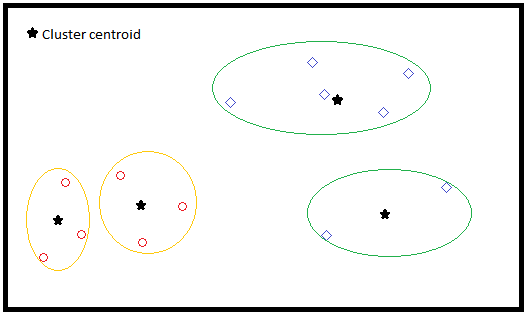
\includegraphics[scale=.6]{chapters/kachra3.png}
  \caption{Clusters}
  
\end{figure}

We have defined positive and negative clusters by having only positive points in positive cluster and negative points in negative cluster. We have proportionate number of positive and negative clusters to as there are number of positive and negative data points. If there are $k_1$ cluster centroids of positive data points and $k_2$ of negative, then $k=k_1+k_2$. ~\cite{maind2014research}

These cluster centroids can now define the closeness of our given sample points.
Each centroid now functions as a feature which says how close is a sample from that centroid.
We use the function
$$e^{-\frac{||x-l||^2}{2\sigma^2}}$$


Our $k$ features can now be defined as
$$f_i=e^{-\frac{||x-l_i||^2}{2\sigma^2}}$$
where $l_i$ is the cluster centroid obtained by k-means algorithm on the tuples that we got from the $X$s of the input data.

This technique not only reduces the risk of underfitting by increasing the number of features, but also deals with the trouble of having a non-separable data in case of SVM.
SVM technique is supposed to be applied on linearly separable data. This technique makes our data linearly separable.
Although kernels can be used in case of SVM, this, infact, is a special case of kernels.

We applied this technique alongside SVM and Logistic Regression.
For SVM with this new technique on Dataset 1, we got the following results.

\begin{center}
\begin{tabular}{| c | c | c | c | c |}
\hline
    & Precision & Recall & f1-score \\
\hline
0 & 0.85 & 0.96 & 0.90 \\
\hline
1 & 0.69 & 0.32 & 0.43 \\
\hline
avg & 0.81 & 0.83 & 0.81 \\
\hline
\end{tabular}
\end{center} 
\begin{center}
The accuracy is 83.11%.
\end{center}

For Logistic Regression with this new technique on Dataset 1, we got the following results.

\begin{center}
\begin{tabular}{| c | c | c | c | c |}
\hline
    & Precision & Recall & f1-score \\
\hline
0 & 0.84 & 0.97 & 0.90 \\
\hline
1 & 0.70 & 0.30 & 0.42 \\
\hline
avg & 0.81 & 0.83 & 0.80 \\
\hline
\end{tabular}
\end{center} 
\begin{center}
The accuracy is 83.03%.
\end{center}

For SVM with this new technique on Dataset 2 after Under-Sampling, we got the following results.

\begin{center}
\begin{tabular}{| c | c | c | c | c |}
\hline
    & Precision & Recall & f1-score \\
\hline
0 & 0.96 & 0.98 & 0.97 \\
\hline
1 & 0.96 & 0.92 & 0.94 \\
\hline
avg & 0.96 & 0.96 & 0.96 \\
\hline
\end{tabular}
\end{center} 
\begin{center}
The accuracy is 95.60%.
\end{center}

For Logistic Regression with this new technique on Dataset 2 after Under-Sampling, we got the following results.

\begin{center}
\begin{tabular}{| c | c | c | c | c |}
\hline
    & Precision & Recall & f1-score \\
\hline
0 & 0.96 & 0.99 & 0.97 \\
\hline
1 & 0.97 & 0.92 & 0.94 \\
\hline
avg & 0.96 & 0.96 & 0.96 \\
\hline
\end{tabular}
\end{center} 
\begin{center}
The accuracy is 96.17%.
\end{center}
